\documentclass{article}

\newcounter{results}
\newcounter{questions}

\def\neg{{\sim}}
\def\Z{\mathbb{Z}}
\def\N{\mathbb{N}}
\def\R{\mathbb{R}}
\def\Q{\mathbb{Q}}
\def\E{\mathbb{E}}
\def\qed{\(\blacksquare\)}
\newcommand{\result}[1]{\stepcounter{results}{\bfseries Result \arabic{results}}: #1}
\newcommand{\question}[1]{\stepcounter{questions}{\bf \arabic{questions}}: #1}
\newenvironment{proof}[2][Proof]{\result{#2}\begin{trivlist} 
    \item[\hskip \labelsep {\sc #1:}]}{\qed\end{trivlist}}
\usepackage{array}
\usepackage{amsmath}
\usepackage{amssymb}
\usepackage{mathtools}
\usepackage{textcomp}
\usepackage{gensymb}
\usepackage{graphicx}
\usepackage{float}
\usepackage{caption}
\usepackage{amsfonts}
\usepackage[margin=1in]{geometry}

\renewcommand{\O}{\(\Omega\)}

\title{Lab 3 Progress Report}
\author{Ryan Coyne \\ Partner: Daniel Albu}

\begin{document}

\maketitle

\section{Introduction}
In this lab, we analyzed a low pass filter, a high pass filter, and an RLC circuit using the Analog Discovery 2. 

\section{Measuring Capacitance}
We built a low pass filter circuit (Figure 1) with the oscilloscope of the AD 2 monitoring the input and output voltages. Using the impedance function in the Waveforms software we measured the series capacitance of the capacitor, C1. We measured 3 capacitors. One was reported to be 100 nF. The second was reported to be 10 nF. The last was reported to be 1 \(\mu\)F. In the diagram, R1 is 10 k\O for the 100 nF capacitor, 100 k\O for the 10 nF capacitor, and 1 k\O for the 1 \(\mu\)F capacitor. We also measured the capacitances using the Mastech MS8268 Multi-Meter. The capacitances were 90.6 nF, 9.2 nF, and 1.13 nF respectively. 

\begin{figure}[H]
    \centering
    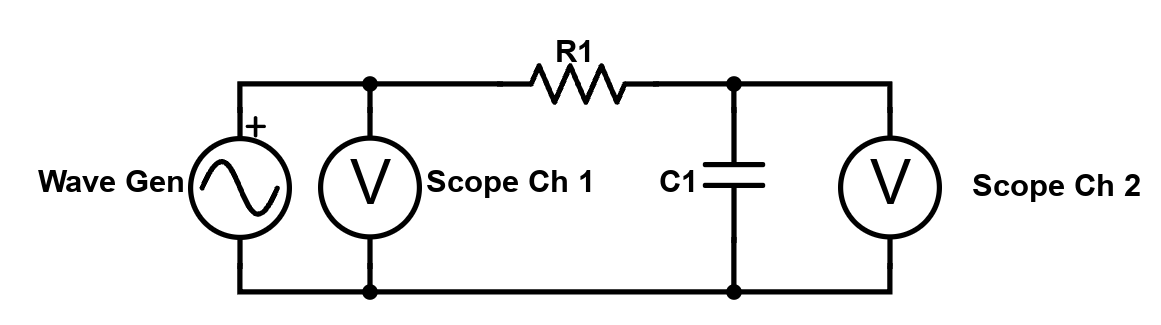
\includegraphics[width = \linewidth]{Scheme-it-export-New-Project-2024-03-04-19-03.png}    
    \caption{Low Pass Filter}
\end{figure}

We conclude that the reported capacitance values of the capacitors are not accurate. The measurements made by the Active Discovery 2 and the multimeter are fairly close. I trust the measurements made by the active discovery more because it reports the capacitance for a particular frequency while the multimeter does not. 

\begin{table}[H]
    \centering
    \begin{tabular}{c|c}
        Frequency (Hz) & Capacitance (nF)\\
        \hline
        1000 & 89.2\\
        500 & 90.1\\
        200 & 91.3\\
        100 & 92.1\\
    \end{tabular}
    \caption{Capacitor 1 Measurements using AD2}
\end{table}

\begin{table}[H]
    \centering
    \begin{tabular}{c|c}
        Frequency (Hz) & Capacitance (nF)\\
        \hline
        1000 & 9.16\\
        500 & 9.21\\
        200 & 9.29\\
        100 & 9.34
    \end{tabular}
    \caption{Capacitor 2 Measurements using AD2}
\end{table}

\begin{table}[H]
    \centering
    \begin{tabular}{c|c}
        Frequency (Hz) & Capacitance (\(\mu\)F)\\
        \hline
        1000 & 1.05\\
        500 & 1.08\\
        200 & 1.15\\
        100 & 1.19
    \end{tabular}
    \caption{Capacitor 3 Measurements using AD2}
\end{table}

\section{Low Pass Filter}
In this part of the lab, we continue to use the previous circuit (Figure 1), with R1=10 k\O\ and C1=100 nF. We sent a square wave from the wave generator through the filter and used the oscilloscope channel 1 to record the input voltage and channel 2 to record the output voltage. The fall time as determined by the AD 2 was 1.87 \(\mu\)s and the rise time as determined by the AD 2 was 1.07 \(\mu\)s

\section{High Pass Filter}


\section{RLC Circuit - Resonance}

\end{document}